\documentclass[11pt]{article}
\usepackage{graphics}
\usepackage{epsfig}
\usepackage{hhline}

\setlength{\textheight}{8.5in}
\setlength{\textwidth}{6in}
\setlength{\oddsidemargin}{0.15in}
\setlength{\parindent}{1pc}
\setlength{\topmargin}{-0.0625in}

% define some macros:
\newcommand{\munged}{{\tt munged}}
\newcommand{\srun}{{\tt srun}}
\newcommand{\scancel}{{\tt scancel}}
\newcommand{\squeue}{{\tt squeue}}
\newcommand{\scontrol}{{\tt scontrol}}
\newcommand{\sinfo}{{\tt sinfo}}
\newcommand{\slurmctld}{{\tt slurmctld}}
\newcommand{\slurmd}{{\tt slurmd}}

\title{SLURM: Simple Linux Utility for Resource Management\thanks{
This document was prepared as an account of work sponsored by an
agency of the United States Government.  Neither the United States
Government nor the University of California nor any of their
employees, makes any warranty, express or implied, or assumes any
legal liability or responsibility for the accuracy, completeness, or
usefulness of any information, apparatus, product, or process
disclosed, or represents that its use would not infringe privately
owned rights. Reference herein to any specific commercial product,
process, or service by trade name, trademark, manufacturer, or
otherwise, does not necessarily constitute or imply its endorsement,
recommendation, or favoring by the United States Government or the
University of California.  The views and opinions of authors expressed
herein do not necessarily state or reflect those of the United States
Government or the University of California, and shall not be used for
advertising or product endorsement purposes.
This work was performed under the auspices of the U. S. Department of
Energy by the University of California, Lawrence Livermore National
Laboratory under Contract No. W-7405-Eng-48. Document UCRL-JC-147996.}}

\author{Morris A. Jette \and Andy B. Yoo \and Mark Grondona}

% We cheat here to easily get the desired allignment 
%\date{\{jette1,mgrondona\}@llnl.gov}
\date{Lawrence Livermore National Laboratory\\
Livermore, CA 94551\\
\{jette1 $\mid$ yoo2 $\mid$ mgrondona\}@llnl.gov}

\begin{document}

\maketitle

\begin{abstract}
A new cluster resource management system called 
Simple Linux Utility Resource Management (SLURM) is developed and 
presented in this paper. SLURM, initially developed for large 
Linux clusters at the Lawrence Livermore National Laboratory (LLNL), 
is a simple cluster manager that can scale to thousands of processors. 
SLURM is designed to be flexible and fault-tolerant and can be ported to 
other clusters of different size and architecture with minimal effort. 
We are certain that SLURM will benefit both users and system architects 
by providing them with a simple, robust, and highly scalable parallel 
job execution environment for their cluster system.
\end{abstract}


\section{Introduction}
Linux clusters, often constructed by using commodity off-the-shelf (COTS) componnets,
have become increasingly populuar as a computing platform for parallel computation
in recent years, mainly due to their ability to deliver a high perfomance-cost ratio.
Researchers have built and used small to medium size clusters for various
applications~\cite{BeowulfWeb,LokiWeb}.
The continuous decrease in the price of the COTS parts in conjunction with
the good scalability of the cluster architecture has now made it feasible to economically
build large-scale clusters with thousands of processors~\cite{MCRWeb,PCRWeb}.

An essential component that is needed to harness such a computer is a
resource management system.
A resource management system (or resource manager) performs such crucial tasks as
scheduling user jobs, monitoring machine and job status, launching user applications, and
managing machine configuration,
An ideal resource manager should be simple, efficient, scalable, fault-tolerant,
and portable.

Unfortunately there are no open-source resource management systems currently available
which satisfy these requirements.
A survey~\cite{Jette02} has revealed that many existing resource managers have poor scalability and fault-tolerance rendering them unsuitable for large clusters having
thousands of processors~\cite{LoadLevelerWeb,LoadLevelerManual}.
While some proprietary cluster managers are suitable for large clusters,
they are typically designed for particular computer systems and/or
interconnects~\cite{RMS,LoadLevelerWeb,LoadLevelerManual}.
Proprietary systems can also be expensive and unavailable in source-code form.
Furthermore, proprietary cluster management functionality is usually provided as a
part of a specific job scheduling system package.
This mandates the use of the given scheduler just to manage a cluster,
even though the scheduler does not necessarily meet the need of organization that hosts the cluster.
Clear separation of the cluster management functionality from scheduling policy is desired.

This observation led us to set out to design a simple, highly scalable, and
portable resource management system.
The result of this effort is Simple Linux Utility Resource Management
(SLURM\footnote{A tip of the hat to Matt Groening and creators of {\em Futurama},
where Slurm is the most popular carbonated beverage in the universe.}).
SLURM was developed with the following design goals:

\begin{itemize}
\item {\em Simplicity}: SLURM is simple enough to allow motivated end-users
to understand its source code and add functionality.  The authors will
avoid the temptation to add features unless they are of general appeal.

\item {\em Open Source}: SLURM is available to everyone and will remain free.
Its source code is distributed under the GNU General Public
License~\cite{GPLWeb}.

\item {\em Portability}: SLURM is written in the C language, with a GNU
{\em autoconf} configuration engine.
While initially written for Linux, other UNIX-like operating systems
should be easy porting targets.
SLURM also supports a general purpose {\em plugin} mechanism, which
permits a variety of different infrastructures to be easily supported.
The SLURM configuration file specifies which set of plugin modules
should be used.

\item {\em Interconnect independence}: SLURM supports UDP/IP based
communication as well as the Quadrics Elan3 and Myrinet interconnects.
Adding support for other interconnects is straightforward and utilizes
the plugin mechanism described above.

\item {\em Scalability}: SLURM is designed for scalability to clusters of
thousands of nodes.
Jobs may specify their resource requirements in a variety of ways
including requirements options and ranges, potentially permitting
faster initiation than otherwise possible.

\item {\em Robustness}: SLURM can handle a variety of failure modes
without terminating workloads, including crashes of the node running
the SLURM controller.
User jobs may be configured to continue execution despite the failure
of one or more nodes on which they are executing.
Nodes allocated to a job are available for reuse as soon as the job(s)
allocated to that node terminate.
If some nodes fail to complete job termination
in a timely fashion due to hardware of software problems, only the
scheduling of those tardy nodes will be effected.

\item {\em Secure}: SLURM employs crypto technology to authenticate
users to services and services to each other with a variety of options
available through the plugin mechanism.
SLURM does not assume that its networks are physically secure,
but does assume that the entire cluster is within a single
administrative domain with a common user base across the
entire cluster.

\item {\em System administrator friendly}: SLURM is configured a
simple configuration file and minimizes distributed state.
Its configuration may be changed at any time without impacting running jobs.
Heterogeneous nodes within a cluster may be easily managed.
SLURM interfaces are usable by scripts and its behavior is highly
deterministic.

\end{itemize}

The main contribution of our work is that we have provided a readily available
tool that anybody can use to efficiently manage clusters of different size and architecture.
SLURM is highly scalable\footnote{It was observed that it took less than five seconds for SLURM to launch a 1900-task job over 950 nodes on recently installed cluster at Lawrence Livermore National Laboratory.}.
The SLURM can be easily ported to any cluster system with minimal effort with its plugin
capability and can be used with any meta-batch scheduler or a Grid resource broker~\cite{Gridbook}
with its well-defined interfaces.

The rest of the paper is organized as follows.
Section 2 describes the architecture of SLURM in detail. Section 3 discusses the services provided by SLURM followed by performance study of
SLURM in Section 4. Brief survey of existing cluster management systems is presented in Section 5.
%Section 6 describes how the SLURM can be used with more sphisticated external schedulers.
Concluding remarks and future development plan of SLURM is given in Section 6.

\section{SLURM Architecture}

As a cluster resource manager, SLURM has three key functions.  First,
it allocates exclusive and/or non-exclusive access to resources to users for 
some duration of time so they can perform work.  Second, it provides 
a framework for starting, executing, and monitoring work  
on the set of allocated nodes.  Finally, it arbitrates 
conflicting requests for resources by managing a queue of pending work.
Users and system administrators interact with SLURM using simple commands.

%Users interact with SLURM through four command line utilities: 
%\srun\ for submitting a job for execution and optionally controlling it
%interactively, 
%\scancel\ for early termination of a pending or running job, 
%\squeue\ for monitoring job queues, and 
%\sinfo\ for monitoring partition and overall system state.
%System administrators perform privileged operations through an additional
%command line utility: {\tt scontrol}.
%
%The central controller daemon, {\tt slurmctld}, maintains the global state 
%and directs operations.
%Compute nodes simply run a \slurmd\ daemon (similar to a remote shell 
%daemon) to export control to SLURM.  
%
%SLURM is not a sophisticated batch system.  
%In fact, it was expressly designed to provide high-performance 
%parallel job management while leaving scheduling decisions to an 
%external entity as will be described later. 

\begin{figure}[tb]
\centerline{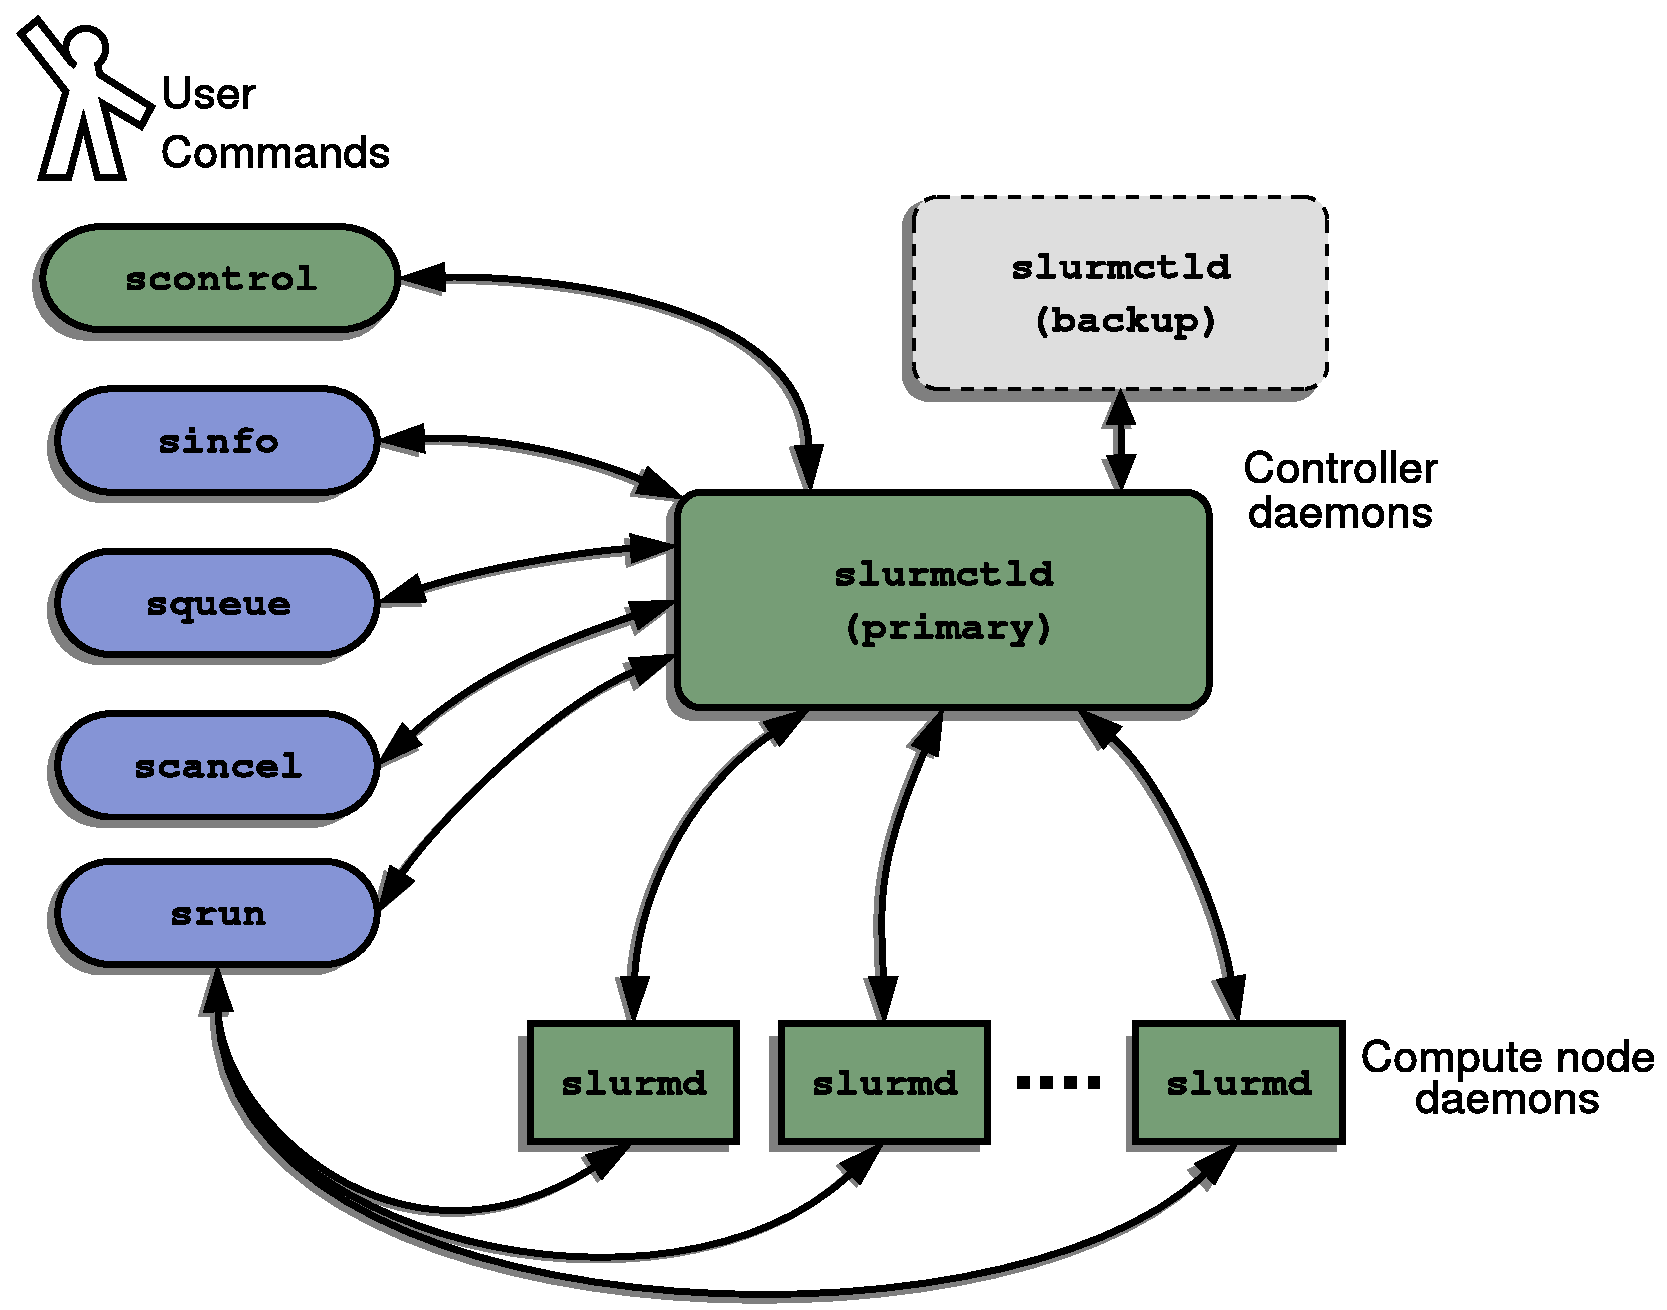
\epsfig{file=../figures/arch.eps,scale=0.40}}
\caption{SLURM Architecture}
\label{arch}
\end{figure}

Figure~\ref{arch} depicts the key components of SLURM. As shown in Figure~\ref{arch},
SLURM consists of a \slurmd\ daemon
running on each compute node, a central \slurmctld\ daemon running on
a management node (with optional fail-over twin), and five command line
utilities,
% {\tt srun}, {\tt scancel}, {\tt sinfo}, {\tt squeue}, and {\tt scontrol}, 
which can run anywhere in the cluster.  

The entities managed by these SLURM daemons include nodes, the
compute resource in SLURM, partitions, which group nodes into
logical disjoint sets, jobs, or allocations of resources assigned
to a user for a specified amount of time, and job steps, which are
sets of tasks within a job.  
Each job is allocated nodes within a single partition. 
Once a job is assigned a set of nodes, the user is able to initiate
parallel work in the form of job steps in any configuration within the
allocation. For instance a single job step may be started which utilizes
all nodes allocated to the job, or several job steps may independently 
use a portion of the allocation.

%\begin{figure}[tcb]
%\centerline{\epsfig{file=../figures/entities.eps,scale=0.7}}
%\caption{SLURM Entities}
%\label{entities}
%\end{figure}
%
%Figure~\ref{entities} further illustrates the interrelation of these
%entities as they are managed by SLURM. The diagram shows a group of
%compute nodes split into two partitions. Partition 1 is running one
%job, with one job step utilizing the full allocation of that job.
%The job in Partition 2 has only one job step using half of the original
%job allocation.
%That job might initiate additional job step(s) to utilize 
%the remaining nodes of its allocation.

\begin{figure}[tb]
\centerline{\epsfig{file=../figures/slurm-arch.eps,scale=0.5}}
\caption{SLURM Architecture - Subsystems}
\label{archdetail}
\end{figure}

Figure~\ref{archdetail} exposes the subsystems that are implemented
within the \slurmd\ and \slurmctld\ daemons.  These subsystems
are explained in more detail below.

\subsection{SLURM Local Daemon (Slurmd)}

The \slurmd\ is a multi-threaded daemon running on each compute node.
It reads the common SLURM configuration file and recovers any 
previously saved state information, 
notifies the controller that it is active, waits for work, 
executes the work, returns status, and waits for more work.  
Since it initiates jobs for other users, it must run with root privilege.
%It also asynchronously exchanges node and job status information with {\tt slurmctld}.  
The only job information it has at any given time pertains to its 
currently executing jobs.
The \slurmd\ performs five major tasks.

\begin{itemize}
\item {\em Machine and Job Status Services}:  Respond to controller 
requests for machine and job state information, and send asynchronous 
reports of some state changes (e.g. \slurmd\ startup) to the controller.

\item {\em Remote Execution}: Start, monitor, and clean up after a set
of processes (typically belonging to a parallel job) as dictated by the
\slurmctld\ daemon or an \srun\ or \scancel\ command. Starting a process may
include executing a prolog program, setting process limits, setting real
and effective user id, establishing environment variables, setting working
directory, allocating interconnect resources, setting core file paths,
initializing the Stream Copy Service, and managing
process groups. Terminating a process may include terminating all members
of a process group and executing an epilog program.

\item {\em Stream Copy Service}: Allow handling of stderr, stdout, and
stdin of remote tasks. Job input may be redirected from a file or files, a
\srun\ process, or /dev/null.  Job output may be saved into local files or
sent back to the \srun\ command. Regardless of the location of stdout or stderr,
all job output is locally buffered to avoid blocking local tasks.

\item {\em Job Control}: Allow asynchronous interaction with the
Remote Execution environment by propagating signals or explicit job
termination requests to any set of locally managed processes.

\end{itemize}

\subsection{SLURM Central Daemon (Slurmctld)}

Most SLURM state information is maintained by the controller, {\tt slurmctld}.
The \slurmctld\ is multi-threaded with independent read and write locks 
for the various data structures to enhance scalability. 
When \slurmctld\ starts, it reads the SLURM configuration file.  
It can also read additional state information
from a checkpoint file generated by a previous execution of {\tt slurmctld}.
Full controller state information is written to 
disk periodically with incremental changes written to disk immediately
for fault-tolerance.  
The \slurmctld\ runs in either master or standby mode, depending on the
state of its fail-over twin, if any.
The \slurmctld\ need not execute with root privilege.
%In fact, it is recommended that a unique user entry be created for 
%executing \slurmctld\ and that user must be identified in the SLURM 
%configuration file as {\tt SlurmUser}.
The \slurmctld\ consists of three major components:

\begin{itemize}
\item {\em Node Manager}: Monitors the state of each node in
the cluster.  It polls {\tt slurmd}'s for status periodically and
receives state change notifications from \slurmd\ daemons asynchronously.
It ensures that nodes have the prescribed configuration before being 
considered available for use.

\item {\em Partition Manager}: Groups nodes into non-overlapping sets called
{\em partitions}. Each partition can have associated with it various job
limits and access controls.  The partition manager also allocates nodes
to jobs based upon node and partition states and configurations. Requests
to initiate jobs come from the Job Manager.  The \scontrol\ may be used
to administratively alter node and partition configurations.

\item {\em Job Manager}: Accepts user job requests and places pending 
jobs in a priority ordered queue. 
The Job Manager is awakened on a periodic basis and whenever there
is a change in state that might permit a job to begin running, such
as job completion, job submission, partition-up transition,
node-up transition, etc.  The Job Manager then makes a pass
through the priority-ordered job queue. The highest priority jobs 
for each partition are allocated resources as possible. As soon as an 
allocation failure occurs for any partition, no lower-priority jobs for 
that partition are considered for initiation. 
After completing the scheduling cycle, the Job Manager's scheduling
thread sleeps.  Once a job has been allocated resources, the Job Manager
transfers necessary state information to those nodes, permitting it 
to commence execution.  When the Job Manager detects that
all nodes associated with a job have completed their work, it initiates
clean-up and performs another scheduling cycle as described above.

\end{itemize}

\section{SLURM Operation and Services}
\subsection{Command Line Utilities}

The command line utilities are the user interface to SLURM functionality.
They offer users access to remote execution and job control. They also 
permit administrators to dynamically change the system configuration. 
These commands all use SLURM APIs which are directly available for 
more sophisticated applications.

\begin{itemize}
\item {\tt scancel}: Cancel a running or a pending job or job step, 
subject to authentication and authorization. This command can also 
be used to send an arbitrary signal to all processes on all nodes 
associated with a job or job step.

\item {\tt scontrol}: Perform privileged administrative commands
such as draining a node or partition in preparation for maintenance. 
Many \scontrol\ functions can only be executed by privileged users.

\item {\tt sinfo}: Display a summary of partition and node information.
A assortment of filtering and output format options are available.

\item {\tt squeue}: Display the queue of running and waiting jobs 
and/or job steps. A wide assortment of filtering, sorting, and output 
format options are available.

\item {\tt srun}: Allocate resources, submit jobs to the SLURM queue,
and initiate parallel tasks (job steps). 
Every set of executing parallel tasks has an associated \srun\ which 
initiated it and, if the \srun\ persists, managing it. 
Jobs may be submitted for batch execution, in which case 
\srun\ terminates after job submission. 
Jobs may also be submitted for interactive execution, where \srun\ keeps 
running to shepherd the running job. In this case, 
\srun\ negotiates connections with remote {\tt slurmd}'s 
for job initiation and to
get stdout and stderr, forward stdin, and respond to signals from the user.
The \srun\ may also be instructed to allocate a set of resources and
spawn a shell with access to those resources.

\end{itemize}

\subsection{Plugins}

In order to make the use of different infrastructures possible, 
SLURM uses a general purpose plugin mechanism. 
A SLURM plugin is a dynamically linked code object which is 
loaded explicitly at run time by the SLURM libraries. 
A plugin provides a customized implemenation of a well-defined
API connected to tasks such as authentication, interconnect fabric, 
task scheduling.
A set of functions is defined for use by all of the different 
infrastructures of a particular variety. 
For example, the authentication plugin must define functions 
such as: 
{\tt slurm\_auth\_activate} to create a credential,
{\tt slurm\_auth\_verify} to verify a credential to 
approve or deny authentication, 
{\tt slurm\_auth\_get\_uid} to get the user ID associated with 
a specific credential.
It also must define the data structure used, a plugin type, 
a plugin version number.
The available plugins are defined in the configuration file.
%When a slurm daemon is initiated, it reads the configuration 
%file to determine which of the available plugins should be used. 
%For example {\em AuthType=auth/authd} says to use the plugin for 
%authd based authentication and {\em PluginDir=/usr/local/lib} 
%identifies the directory in which to find the plugin.

\subsection{Communications Layer}

SLURM presently uses Berkeley sockets for communications. 
However, we anticipate using the plugin mechanism to easily 
permit use of other communications layers. 
At LLNL we are using an Ethernet for SLURM communications and 
the Quadrics Elan switch exclusively for user applications. 
The SLURM configuration file permits the identification of each 
node's hostname as well as its name to be used for communications. 
%In the case of a control machine known as {\em mcri} to be 
%communicated with using the name {\em emcri} (say to indicate 
%an ethernet communications path), this is represented in the 
%configuration file as {\em ControlMachine=mcri ControlAddr=emcri}.
%The name used for communication is the same as the hostname unless 
%%otherwise specified.

While SLURM is able to manage 1000 nodes without difficulty using 
sockets and Ethernet, we are reviewing other communication 
mechanisms which may offer improved scalability. 
One possible alternative is STORM\cite{STORM2001}. 
STORM uses the cluster interconnect and Network Interface Cards to 
provide high-speed communications including a broadcast capability. 
STORM only supports the Quadrics Elan interconnnect at present, 
but does offer the promise of improved performance and scalability. 

\subsection{Security}

SLURM has a simple security model: 
Any user of the cluster may submit parallel jobs to execute and cancel
his own jobs.  Any user may view SLURM configuration and state
information.  
Only privileged users may modify the SLURM configuration,
cancel any jobs, or perform other restricted activities.  
Privileged users in SLURM include the users {\em root} 
and {\tt SlurmUser} (as defined in the SLURM configuration file). 
If permission to modify SLURM configuration is 
required by others, set-uid programs may be used to grant specific
permissions to specific users.

We presently support three authentication mechanisms via plugins: 
{\tt authd}\cite{Authd2002}, {\tt munged} and {\tt none}. 
A plugin can easily be developed for Kerberos or authentication 
mechanisms as desired.
The \munged\ implementation is described below.
A \munged\ daemon running as user {\em root} on each node confirms the 
identify of the user making the request using the {\tt getpeername} 
function and generates a credential. 
The credential contains a user ID, 
group ID, time-stamp, lifetime, some pseudo-random information, and 
any user supplied information. The \munged\ uses a private key to 
generate a Message Authentication Code (MAC) for the credential.
The \munged\ then uses a public key to symmetrically encrypt 
the credential including the MAC. 
SLURM daemons and programs transmit this encrypted 
credential with communications. The SLURM daemon receiving the message 
sends the credential to \munged\ on that node. 
The \munged\ decrypts the credential using its private key, validates it 
and returns the user ID and group ID of the user originating the 
credential.
The \munged\ prevents replay of a credential on any single node 
by recording credentials that have already been authenticated.
In SLURM's case, the user supplied information includes node 
identification information to prevent a credential from being 
used on nodes it is not destined for.

When resources are allocated to a user by the controller, a 
{\em job step credential} is generated by combining the user ID, job ID, 
step ID, the list of resources allocated (nodes), and the credential
lifetime. This job step credential is encrypted with 
a \slurmctld\ private key. This credential 
is returned to the requesting agent ({\tt srun}) along with the
allocation response, and must be forwarded to the remote {\tt slurmd}'s 
upon job step initiation. \slurmd\ decrypts this credential with the
\slurmctld 's public key to verify that the user may access
resources on the local node. \slurmd\ also uses this job step credential 
to authenticate standard input, output, and error communication streams. 

%Access to partitions may be restricted via a {\em RootOnly} flag.  
%If this flag is set, job submit or allocation requests to this 
%partition are only accepted if the effective user ID originating 
%the request is a privileged user. 
%The request from such a user may submit a job as any other user. 
%This may be used, for example, to provide specific external schedulers
%with exclusive access to partitions.  Individual users will not be 
%permitted to directly submit jobs to such a partition, which would 
%prevent the external scheduler from effectively managing it.  
%Access to partitions may also be restricted to users who are 
%members of specific Unix groups using a {\em AllowGroups} specification.

\subsection{Job Initiation}

There are three modes in which jobs may be run by users under SLURM. The
first and most simple is {\em interactive} mode, in which stdout and
stderr are displayed on the user's terminal in real time, and stdin and
signals may be forwarded from the  terminal transparently to the remote
tasks. The second is {\em batch} mode, in which the job is
queued until the request for resources can be satisfied, at which time the
job is run by SLURM as the submitting user. In {\em allocate} mode,
a job is allocated to the requesting user, under which the user may
manually run job steps via a script or in a sub-shell spawned by \srun .

\begin{figure}[tb]
\centerline{\epsfig{file=../figures/connections.eps,scale=0.5}}
\caption{\small Job initiation connections overview. 1. The \srun\ connects to
         \slurmctld\ requesting resources. 2. \slurmctld\ issues a response,
         with list of nodes and job credential. 3. The \srun\ opens a listen
         port for every task in the job step, then sends a run job step
         request to \slurmd . 4. \slurmd 's initiate job step and connect
         back to \srun\ for stdout/err. }
\label{connections}
\end{figure}

Figure~\ref{connections} gives a high-level depiction of the connections
that occur between SLURM components during a general interactive job
startup.
The \srun\ requests a resource allocation and job step initiation from the {\tt slurmctld},
which responds with the job ID, list of allocated nodes, job credential.
if the request is granted.
The \srun\ then initializes listen ports for each
task and sends a message to the {\tt slurmd}'s on the allocated nodes requesting
that the remote processes be initiated. The {\tt slurmd}'s begin execution of
the tasks and connect back to \srun\ for stdout and stderr. This process and
the other initiation modes are described in more detail below.

\subsubsection{Interactive mode initiation}

\begin{figure}[tb]
\centerline{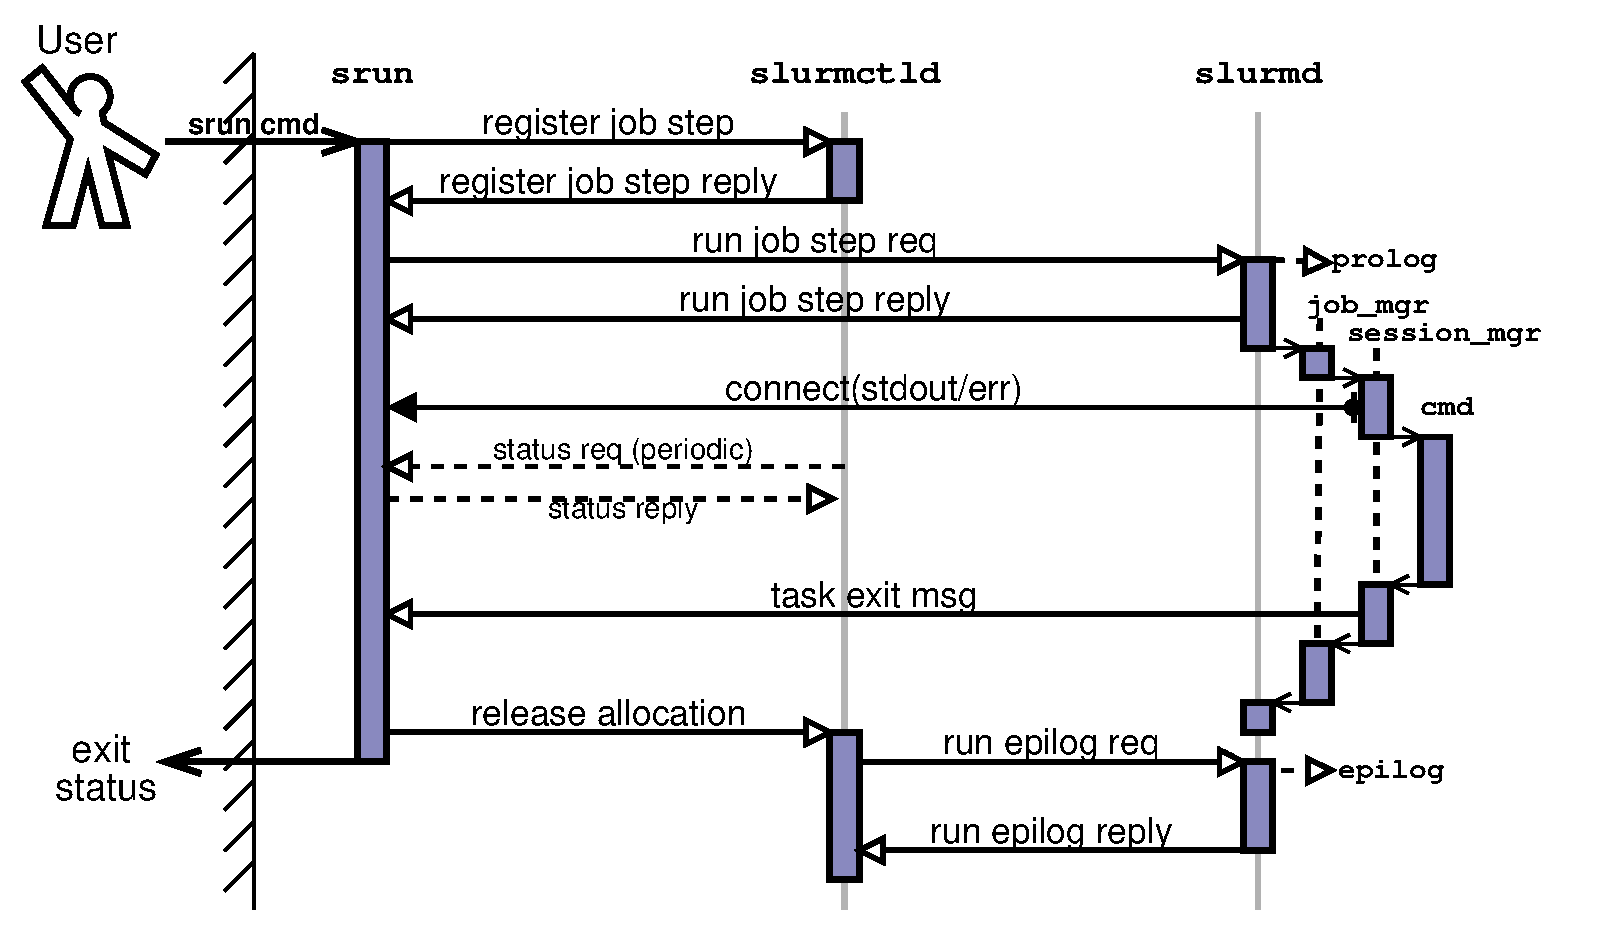
\epsfig{file=../figures/interactive-job-init.eps,scale=0.5} }
\caption{\small Interactive job initiation. \srun\ simultaneously allocates
nodes
         and a job step from \slurmctld\ then sends a run request to all
         \slurmd 's in job. Dashed arrows indicate a periodic request that
         may or may not occur during the lifetime of the job.}
\label{init-interactive}
\end{figure}

Interactive job initiation is illustrated in Figure~\ref{init-interactive}.
The process begins with a user invoking \srun\ in interactive mode.
In Figure~\ref{init-interactive}, the user has requested an interactive
run of the executable ``{\tt cmd}'' in the default partition.

After processing command line options, \srun\ sends a message to
\slurmctld\ requesting a resource allocation and a job step initiation.
This message simultaneously requests an allocation (or job) and a job step.
The \srun\ waits for a reply from {\tt slurmctld}, which may not come instantly
if the user has requested that \srun\ block until resources are available.
When resources are available
for the user's job, \slurmctld\ replies with a job step credential, list of
nodes that were allocated, cpus per node, and so on. The \srun\ then sends
a message each \slurmd\ on the allocated nodes requesting that a job
step be initiated. The \slurmd 's verify that the job is valid using
the forwarded job step credential and then respond to \srun .

Each \slurmd\ invokes a job thread to handle the request, which in turn
invokes a task thread for each requested task. The task thread connects
back to a port opened by \srun\ for stdout and stderr. The host and
port for this connection is contained in the run request message sent
to this machine by \srun . Once stdout and stderr have successfully
been connected, the task thread takes the necessary steps to initiate
the user's executable on the node, initializing environment, current
working directory, and interconnect resources if needed.

Once the user process exits, the task thread records the exit status and
sends a task exit message back to \srun . When all local processes
terminate, the job thread exits. The \srun\ process either waits
for all tasks to exit, or attempt to clean up the remaining processes
some time after the first task exits.
Regardless, once all
tasks are finished, \srun\ sends a message to the \slurmctld\ releasing
the allocated nodes, then exits with an appropriate exit status.

When the \slurmctld\ receives notification that \srun\ no longer needs
the allocated nodes, it issues a request for the epilog to be run on each of
the \slurmd 's in the allocation. As \slurmd 's report that the epilog ran
successfully, the nodes are returned to the partition.


\subsubsection{Batch mode initiation}

\begin{figure}[tb]
\centerline{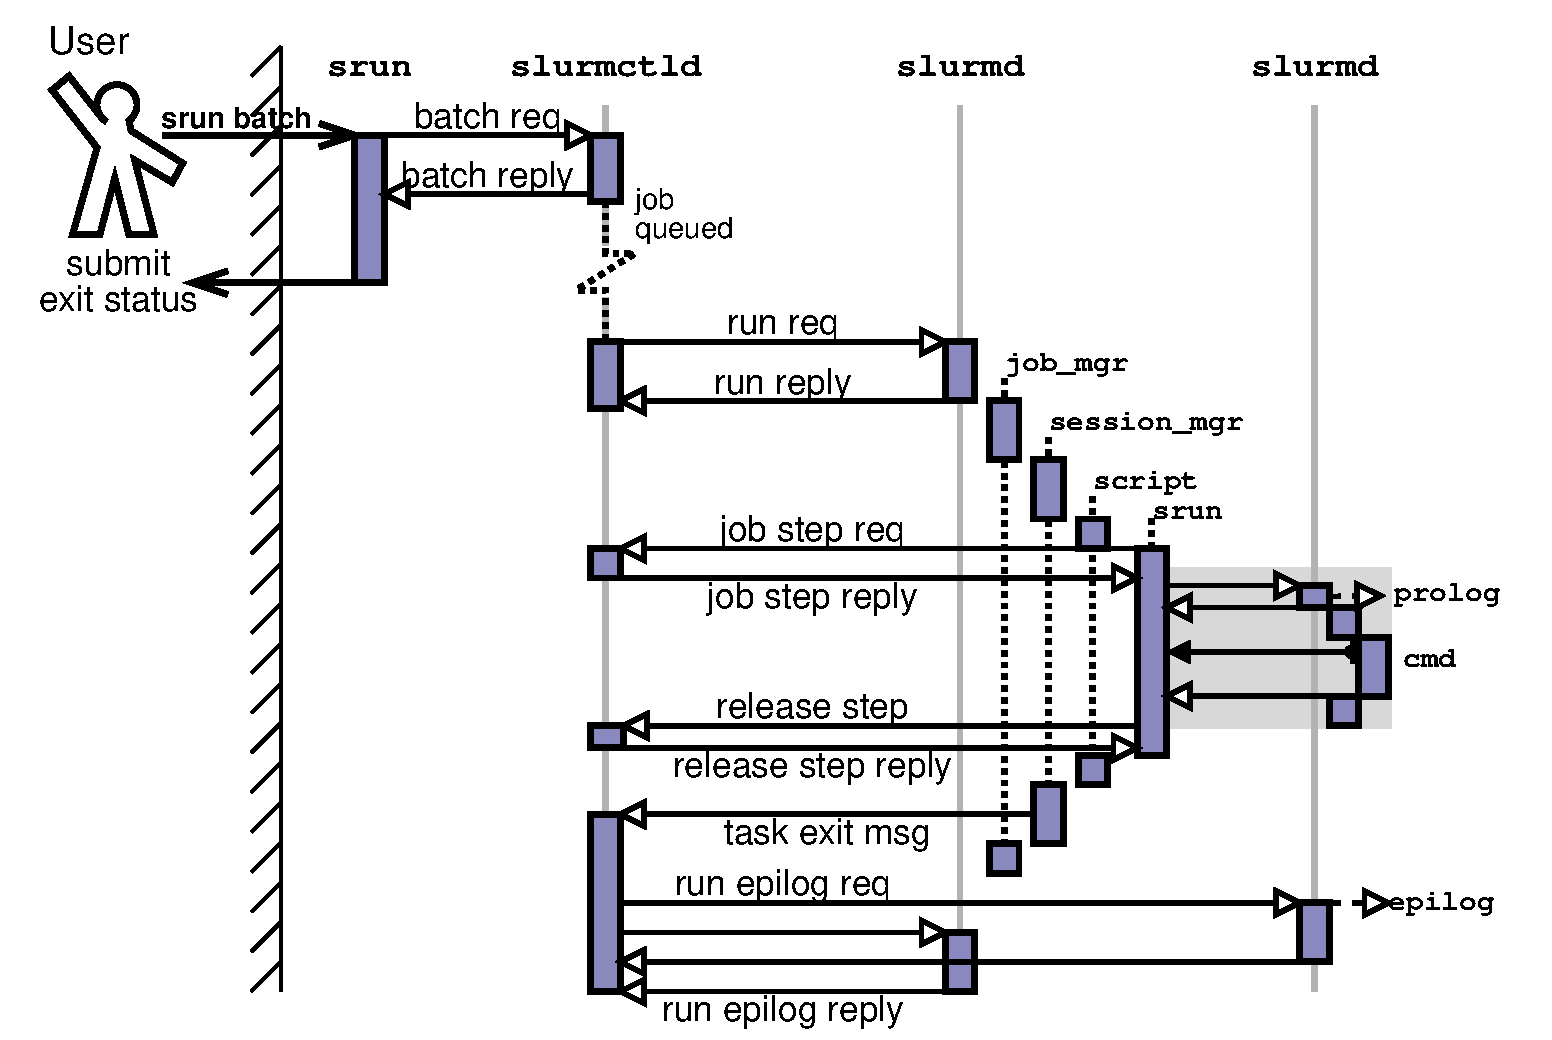
\epsfig{file=../figures/queued-job-init.eps,scale=0.5} }
\caption{\small Queued job initiation.
         \slurmctld\ initiates the user's job as a batch script on one node.
         Batch script contains an srun call which initiates parallel tasks
         after instantiating job step with controller. The shaded region is
         a compressed representation and is illustrated in more detail in the
         interactive diagram (Figure~\ref{init-interactive}).}
\label{init-batch}
\end{figure}

Figure~\ref{init-batch} illustrates the initiation of a batch  job in SLURM.
Once a batch job is submitted, \srun\ sends a batch job request
to \slurmctld\ that contains the input/output location for the job, current
working directory, environment, requested number of nodes. The
\slurmctld\ queues the request in its priority ordered queue.

Once the resources are available and the job has a high enough priority,
\slurmctld\ allocates the resources to the job and contacts the first node
of the allocation requesting that the user job be started. In this case,
the job may either be another invocation of \srun\ or a {\em job script} which
may have multiple invocations of \srun\ within it. The \slurmd\ on the remote
node responds to the run request, initiating the job thread, task thread,
and user script. An \srun\ executed from within the script detects that it
has access to an allocation and initiates a job step on some or all of the
nodes within the job.

Once the job step is complete, the \srun\ in the job script notifies the
\slurmctld\, and terminates. The job script continues executing and may
initiate further job steps. Once the job script completes, the task
thread running the job script collects the exit status and sends a task exit
message to the \slurmctld . The \slurmctld\ notes that the job is complete
and requests that the job epilog be run on all nodes that were allocated.
As the \slurmd 's respond with successful completion of the epilog,
the nodes are returned to the partition.

\subsubsection{Allocate mode initiation}

\begin{figure}[tb]
\centerline{\epsfig{file=../figures/allocate-init.eps,scale=0.5} }
\caption{\small Job initiation in allocate mode. Resources are allocated and
         \srun\ spawns a shell with access to the resources. When user runs
         an \srun\ from within the shell, the a job step is initiated under
         the allocation.}
\label{init-allocate}
\end{figure}

In allocate mode, the user wishes to allocate a job and interactively run
job steps under that allocation. The process of initiation in this mode
is illustrated in Figure~\ref{init-allocate}. The invoked \srun\ sends
an allocate request to \slurmctld , which, if resources are available,
responds with a list of nodes allocated, job id, etc. The \srun\
process spawns a shell on the user's terminal with access to the
allocation, then waits for the shell to exit at which time the job
is considered complete.

An \srun\ initiated within the allocate sub-shell recognizes that it
is running under an allocation and therefore already within a job. Provided
with no other arguments, \srun\ started in this manner initiates a job
step on all nodes within the current job. However, the user may select
a subset of these nodes implicitly.

An \srun\ executed from the sub-shell reads the environment and
user options, then notify the controller that it is starting a job step
under the current job. The \slurmctld\ registers the job step and responds
with a job credential. The \srun\ then initiates the job step using the same
general method as described in the section on interactive job initiation.

When the user exits the allocate sub-shell, the original \srun\ receives
exit status, notifies \slurmctld\ that the job is complete, and exits.
The controller runs the epilog on each of the allocated nodes, returning
nodes to the partition as they complete the epilog.

\section{Related Work}
\subsection*{Portable Batch System (PBS)}

The Portable Batch System (PBS)~\cite{PBS}
is a flexible batch queuing and 
workload management system originally developed by Veridian Systems 
for NASA.  It operates on networked, multi-platform UNIX environments, 
including heterogeneous clusters of workstations, supercomputers, and 
massively parallel systems. PBS was developed as a replacement for 
NQS (Network Queuing System) by many of the same people.

PBS supports sophisticated scheduling logic (via the Maui 
Scheduler\footnote{http://superclustergroup.org/maui}). 
PBS spawn's daemons on each 
machine to shepherd the job's tasks.
It provides an interface for administrators to easily 
interface their own scheduling modules.  PBS can support 
long delays in file staging with retry.  Host 
authentication is provided by checking port numbers (low ports numbers are only 
accessible to user root).  Credential service is used for user authentication. 
It has the job prolog and epilog feature.
PBS Supports 
high priority queue for smaller "interactive" jobs.  Signal to daemons 
causes current log file to be closed, renamed with 
time-stamp, and a new log file created.

Although the PBS is portable and has broad user base, it has following drawbacks.
First, PBS is implementted using single thread and hence exhibits poor performance
especially when a compute node in the system dies in which case the PBS
tries to contact down nodes, while other activities must wait. Second, PBS
has weak mechanism for starting and cleaning up parallel jobs. Finally, the PBS
has very poor scalability and is not suitable for large clusters.
%Specific complaints about PBS from members of the OSCAR group (Jeremy Enos, 
%Jeff Squyres, Tim Mattson):
%\begin{itemize}
%\item Sensitivity to hostname configuration on the server; improper 
%      configuration results in hard to diagnose failure modes.  Once 
%      configuration is correct, this issue disappears.
%\item When a compute node in the system dies, everything slows down.  
%      PBS is single-threaded and continues to try to contact down nodes,
%      while other activities like scheduling jobs, answering qsub/qstat 
%      requests, etc., have to wait for a complete timeout cycle before being
%      processed.
%\item Default scheduler is just FIFO, but Maui can be plugged in so this
%      is not a big issue.
%\item Weak mechanism for starting/cleaning up parallel jobs (pbsdsh).
%      When a job is killed, pbsdsh kills the processes it started, but
%      if the process doesn't die on the first shot it may continue on.
%\item PBS server continues to mark specific nodes offline, even though they 
%      are healthy.  Restarting the server fixes this.
%\item Lingering jobs.  Jobs assigned to nodes, and then bounced back to the 
%      queue for any reason, maintain their assignment to those nodes, even 
%      if another job had already started on them.  This is a poor clean up 
%      issue.
%\item When the PBS server process is restarted, it puts running jobs at risk.
%\item Poor diagnostic messages.  This problem can be as serious as ANY other 
%      problem.  This problem makes small, simple problems turn into huge 
%      turmoil occasionally.  For example, the variety of symptoms that arise 
%      from improper hostname configuration.  All the symptoms that result are 
%      very misleading to the real problem.
%\item Rumored to have problems when the number of jobs in the queues gets
%      large.
%\item Scalability problems on large systems.
%\item Non-portable to Windows
%\item Source code is a mess and difficult for others (e.g. the open source
%      community) to improve/expand.
%\item Licensing problems (see below).
%\end{itemize}
%The one strength mentioned is PBS's portability and broad user base.
%
%PBS is owned by Veridian and is released as three separate products with
%different licenses: {\em PBS Pro} is a commercial product sold by Veridian;
%{\em OpenPBS} is an pseudo open source version of PBS that requires 
%registration; and
%{\em PBS} is a GPL-like, true open source version of PBS.
%
%Bug fixes go into PBS Pro.  When a major revision of PBS Pro comes out,
%the previous version of PBS Pro becomes OpenPBS, and the previous version
%of OpenPBS becomes PBS.  The delay getting bug fixes (some reported by the
%open source community) into the true open source version of PBS is the source
%of some frustration.

\subsection*{Maui Scheduler}

Maui Scheduler~\cite{Maui}
is an advance reservation HPC batch scheduler for use with SP, 
O2K, and UNIX/Linux clusters. It is widely used to extend the 
functionality of PBS and LoadLeveler

\subsection*{Distributed Production Control System (DPCS)}

The Distributed Production Control System (DPCS)~\cite{DPCS}
is a resource manager developed at Lawrence Livermore National Laboratory (LLNL). 
The DPCS provides basic data collection and reporting
mechanisms for prject-level, near real-time accounting and resource allocation
to customers with established limits per customers' organization budgets,
In addition, the DPCS evenly distributes workload across available computers
and supports dynamic reconfiguration and graceful degradation of service to prevent
overuse of a computer where not authorized.
%DPCS is (or will soon be) open source, although its use is presently 
%confined to LLNL. The development of DPCS began in 1990 and it has 
%evolved into a highly scalable and fault-tolerant meta-scheduler 
%operating on top of LoadLeveler, RMS, and NQS. DPCS provides: 
%\begin{itemize}
%\item Basic data collection and reporting mechanisms for project-level, 
%      near real-time accounting.
%\item Resource allocation to customers with established limits per 
%      customers' organizational budgets. 
%\item Proactive delivery of services to organizations that are relatively 
%      underserviced using a fair-share resource allocation scheme.
%\item Automated, highly flexible system with feedback for proactive delivery 
%      of resources.
%\item Even distribution of the workload across available computers.
%\item Flexible prioritization of production workload, including "run on demand."
%\item Dynamic reconfiguration and re-tuning.
%\item Graceful degradation in service to prevent overuse of a computer where 
%      not authorized.
%\end{itemize}

While DPCS does have these attractive characteristics, it supports only a 
limited number of computer systems: IBM RS/6000 and SP, Linux with RMS, 
Sun Solaris, and Compaq Alpha. DPCS also lacks commercial support.

\subsection*{LoadLeveler}

LoadLeveler~cite{LoadLevelerManual,LoadLevelerWeb} 
is a proprietary batch system and parallel job manager by 
IBM. LoadLeveler supports few non-IBM systems. Very primitive 
scheduling software exists and other software is required for reasonable 
performance such as Maui Scheduler and DPCS. 
The LoadLeveler is simple and very flexible queue and job class structure is available 
operating in "matrix" fashion. 
The biggest problem of the LoadLeveler is its extremely poor scalability. It was observed that 
it took more than 20 minutes to start-up a 512-task job using LoadLeveler on one of
the IBM SP machines at LLNL.
In addition, all jobs must be initiated through the LoadLeveler, and a special version of
MPI is requested to run a parallel job.
%Many configuration files exist with signals to 
%daemons used to update configuration (like LSF, good). All jobs must 
%be initiated through LoadLeveler (no real "interactive" jobs, just 
%high priority queue for smaller jobs). Job accounting is only available 
%on termination (very bad for long-running jobs). Good status 
%information on nodes and LoadLeveler daemons is available. LoadLeveler 
%allocates jobs either entire nodes or shared nodes ,depending upon configuration.
%
%A special version of MPI is required. LoadLeveler allocates 
%interconnect resources, spawns the user's processes, and manages the 
%job afterwards. Daemons also monitor the switch and node health using 
%a "heart-beat monitor." One fundamental problem is that when the 
%"Central Manager" restarts, it forgets about all nodes and jobs. They 
%appear in the database only after checking in via the heartbeat. It 
%needs to periodically write state to disk instead of doing 
%"cold-starts" after the daemon fails, which is rare. It has the job 
%prolog and epilog feature, which permits us to enable/disable logins 
%and remove stray processes.
%
%LoadLeveler evolved from Condor, or what was Condor a decade ago. 
%While I am less familiar with LSF and Condor than LoadLeveler, they 
%all appear very similar with LSF having the far more sophisticated 
%scheduler. We should carefully review their data structures and 
%daemons before designing our own.
%
\subsection*{Load Sharing Facility (LSF)}

LSF~\cite{LSF}
is a proprietary batch system and parallel job manager by 
Platform Computing. Widely deployed on a wide variety of computer 
architectures, it has sophisticated scheduling software including 
fair-share, backfill, consumable resources, an job preemption and 
very flexible queue structure.
It also provides good status information on nodes and LSF daemons.
The LSF share many of its shortcomings with the LoadLeveler: job initiation only
through LSF, requirement of a spwcial MPI library, etc.
%Limits are available on both a per process bs per-job  
%basis. Time limits include CPU time and wall-clock time. Many 
%configuration files with signals to daemons used to update 
%configuration (like LoadLeveler, good). All jobs must be initiated 
%through LSF to be accounted for and managed by LSF ("interactive" 
%jobs can be executed through a high priority queue for 
%smaller jobs). Job accounting only available in near real-time (important 
%for long-running jobs). Jobs initiated from same directory as 
%submitted from (not good for computer centers with diverse systems 
%under LSF control). Good status information on nodes and LSF daemons. 
%Allocates jobs either entire nodes or shared nodes depending upon 
%configuration.
%
%A special version of MPI is required. LSF allocates interconnect 
%resources, spawns the user's processes, and manages the job 
%afterwards. While I am less familiar with LSF than LoadLeveler, they 
%appear very similar with LSF having the far more sophisticated 
%scheduler. We should carefully review their data structures and 
%daemons before designing our own.


\subsection*{Condor}

Condor~\cite{Condor,Litkow88,Basney97}
is a batch system and parallel job manager 
developed by the University of Wisconsin. 
Condor was the basis for IBM's LoadLeveler and both share very similar 
underlying infrastructure. Condor has a very sophisticated checkpoint/restart 
service that does not rely upon kernel changes, but a variety of 
library changes (which prevent it from being completely general). The 
Condor checkpoint/restart service has been integrated into LSF, 
Codine, and DPCS. Condor is designed to operate across a 
heterogeneous environment, mostly to harness the compute resources of 
workstations and PCs. It has an interesting "advertising" service. 
Servers advertise their available resources and consumers advertise 
their requirements for a broker to perform matches. The checkpoint 
mechanism is used to relocate work on demand (when the "owner" of a 
desktop machine wants to resume work).



\subsection*{Memory Channel}

Memory Channel is a high-speed interconnect developed by 
Digital/Compaq with related software for parallel job execution. 
Special version of MPI required. The application spawns tasks on 
other nodes. These tasks connect themselves to the high speed 
interconnect. No system level tool to spawns the tasks, allocates 
interconnect resources, or otherwise manages the parallel job (Note: 
This is sometimes a problem when jobs fail, requiring system 
administrators to release interconnect resources. There are also 
performance problems related to resource sharing).

\subsection*{Linux PAGG Process Aggregates}


PAGG~\cite{PAGG}
consists of modifications to the linux kernel that allows
developers to implement Process AGGregates as loadable kernel modules.
A process aggregate is defined as a collection of processes that are
all members of the same set. A set would be implemented as a container
for the member processes. For instance, process sessions and groups
could have been implemented as process aggregates.

\subsection*{Beowulf Distributed Process Space (BPROC)}


The Beowulf Distributed Process Space 
(BPROC)
is set of kernel
modifications, utilities and libraries which allow a user to start
processes on other machines in a Beowulf-style cluster~\cite{BProc}.  Remote
processes started with this mechanism appear in the process table
of the front end machine in a cluster. This allows remote process
management using the normal UNIX process control facilities. Signals
are transparently forwarded to remote processes and exit status is
received using the usual wait() mechanisms.

%\subsection{xcat}
%
%Presumably IBM's suite of cluster management software 
%(xcat\footnote{http://publib-b.boulder.ibm.com/Redbooks.nsf/RedbookAbstracts/sg246041.html})
%includes a batch system.  Look into this.
%
%\subsection{CPLANT}
%
%CPLANT\footnote{http://www.cs.sandia.gov/cplant/} includes
%Parallel Job Launcher, Compute Node Daemon Process,
%Compute Node Allocator, Compute Node Status Tool.
%
%\subsection{NQS} 
%
%NQS\footnote{http://umbc7.umbc.edu/nqs/nqsmain.html}, 
%the Network Queueing System, is a serial batch system.
%
\subsection*{LAM / MPI}

Local Area Multicomputer (LAM)~\cite{LAM}
is an MPI programming environment and development system for heterogeneous 
computers on a network. 
With LAM, a dedicated cluster or an existing network
computing infrastructure can act as one parallel computer solving
one problem.  LAM features extensive debugging support in the
application development cycle and peak performance for production
applications. LAM features a full implementation of the MPI
communication standard.

%\subsection{MPICH}
%
%MPICH\footnote{http://www-unix.mcs.anl.gov/mpi/mpich/}
%is a freely available, portable implementation of MPI,
%the Standard for message-passing libraries.
%
%\subsection{Quadrics RMS}
%
%Quadrics
%RMS\footnote{http://www.quadrics.com/downloads/documentation/}
%(Resource Management System) is a cluster management system for 
%Linux and Tru64 which supports the
%Elan3 interconnect.  
%
%\subsection{Sun Grid Engine}
%
%SGE\footnote{http://www.sun.com/gridware/} is now proprietary.
%
%
%\subsection{SCIDAC}
%
%The Scientific Discovery through Advanced Computing (SciDAC) 
%project\footnote{http://www.scidac.org/ScalableSystems}
%has a Resource Management and Accounting working group
%and a white paper\cite{Res2000}. Deployment of a system with 
%the required fault-tolerance and scalability is scheduled 
%for June 2006.
%
%\subsection{GNU Queue}
%
%GNU Queue\footnote{http://www.gnuqueue.org/home.html}.
%
%\subsection{Clubmask}
%Clubmask\footnote{http://clubmask.sourceforge.net} is based on bproc.
%Separate queueing system?
%
%\subsection{SQMX}
%Part of the SCE Project\footnote{http://www.opensce.org/}, 
%SQMX\footnote{http://www.beowulf.org/pipermail/beowulf-announce/2001-January/000086.html} is worth taking a look at.

%\section{Scheduling Infrastructure}

Scheduling parallel computers is a very complex matter.
Several good public domain schedulers exist with the most
popular being the Maui Scheduler\cite{Jackson2001,Maui2002}.
The scheduler used at our site, DPCS\cite{DPCS2002}, is quite
sophisticated and has over 150,000 lines of code.
We felt no need to address scheduling issues within SLURM, but
have instead developed a resource manager with a rich set of
application programming interfaces (APIs) and the flexibility
to satisfy the needs of others working on scheduling issues.
SLURM's default scheduler implements First-In First-Out (FIFO).
An external entity can establish a job's initial priority
through a plugin.
An external scheduler may also submit, signal, hold, reorder and
terminate jobs via the API.

\subsection{Resource Specification}

The \srun\ command and corresponding API have a wide of resource
specifications available. The \srun\ resource specification options
are described below.

\subsubsection{Geometry Specification}

These options describe how many nodes and tasks are needed as
well as describing the distribution of tasks across the nodes.

\begin{itemize}
\item {\tt cpus-per-task=<number>}:
Specifies the number of processors cpus) required for each task
(or process) to run.
This may be useful if the job is multithreaded and requires more
than one cpu per task for optimal performance.
The default is one cpu per process.

\item {\tt nodes=<number>[-<number>]}:
Specifies the number of nodes required by this job.
The node count may be either a specific value or a minimum and maximum
node count separated by a hyphen.
The partition's node limits supersede those of the job.
If a job's node limits are completely outside of the range permitted
for it's associated partition, the job will be left in a PENDING state.
The default is to allocate one cpu per process, such that nodes with
one cpu will run one task, nodes with 2 cpus will run two tasks, etc.
The distribution of processes across nodes may be controlled using
this option along with the {\tt nproc} and {\tt cpus-per-task} options.

\item {\tt nprocs=<number>}:
Specifies the number of processes to run.
Specification of the number of processes per node may be achieved
with the {\tt cpus-per-task} and {\tt nodes} options.
The default is one process per node unless {\tt cpus-per-task}
explicitly specifies otherwise.

\end{itemize}

\subsubsection{Constraint Specification}

These options describe what configuration requirements of the nodes
which can be used.

\begin{itemize}

\item {\tt constraint=list}:
Specify a list of constraints. The list of constraints is
a comma separated list of features that have been assigned to the
nodes by the slurm administrator. If no nodes have the requested
feature, then the job will be rejected.

\item {\tt contiguous=[yes|no]}:
demand a contiguous range of nodes. The default is "yes".

\item {\tt mem=<number>}:
Specify a minimum amount of real memory per node (in megabytes).

\item {\tt mincpus=<number>}:
Specify minimum number of cpus per node.

\item {\tt partition=name}:
Specifies the partition to be used.
There will be a default partition specified in the SLURM configuration file.

\item {\tt tmp=<number>}:
Specify a minimum amount of temporary disk space per node (in megabytes).

\item {\tt vmem=<number>}:
Specify a minimum amount of virtual memory per node (in megabytes).

\end{itemize}

\subsubsection{Other Resource Specification}

\begin{itemize}

\item {\tt batch}:
Submit in "batch mode."
srun will make a copy of the executable file (a script) and submit therequest for execution when resouces are available.
srun will terminate after the request has been submitted.
The executable file will run on the first node allocated to the
job and must contain srun commands to initiate parallel tasks.

\item {\tt exclude=[filename|node\_list]}:
Request that a specific list of hosts not be included in the resources
allocated to this job. The host list will be assumed to be a filename
if it contains a "/"character. If some nodes are suspect, this option
may be used to avoid using them.

\item {\tt immediate}:
Exit if resources are not immediately available.
By default, the request will block until resources become available.

\item {\tt nodelist=[filename|node\_list]}:
Request a specific list of hosts. The job will contain at least
these hosts. The list may be specified as a comma-separated list of
hosts, a range of hosts (host[1-5,7,...] for example), or a filename.
The host list will be assumed to be a filename if it contains a "/"
character.

\item {\tt overcommit}:
Overcommit resources.
Normally the job will not be allocated more than one process per cpu.
By specifying this option, you are explicitly allowing more than one process
per cpu.

\item {\tt share}:
The job can share nodes with other running jobs. This may result in faster job
initiation and higher system utilization, but lower application performance.

\item {\tt time=<number>}:
Establish a time limit to terminate the job after the specified number of
minutes. If the job's time limit exceed's the partition's time limit, the
job will be left in a PENDING state. The default value is the partition's
time limit. When the time limit is reached, the job's processes are sent
SIGXCPU followed by SIGKILL. The interval between signals is configurable.

\end{itemize}

All parameters may be specified using single letter abbreviations
("-n" instead of "--nprocs=4").
Environment variable can also be used to specify many parameters.
Environment variable will be set to the actual number of nodes and
processors allocated
In the event that the node count specification is a range, the
application could inspect the environment variables to scale the
problem appropriately.
To request four processes with one cpu per task the command line would
look like this: {\em srun --nprocs=4 --cpus-per-task=1 hostname}.
Note that if multiple resource specifications are provided, resources
will be allocated so as to satisfy the all specifications.
For example a request with the specification {\tt nodelist=dev[0-1]}
and {\tt nodes=4} may be satisfied with nodes {\tt dev[0-3]}.

\subsection{The Maui Scheduler and SLURM}

{\em The integration of the Maui Scheduler with SLURM was
just beginning at the time this paper was written. Full
integration is anticipated by the time of the conference.
This section will be modified as needed based upon that
experience.}

The Maui Scheduler is integrated with SLURM through the
previously described plugin mechanism.
The previously described SLURM commands are used for
all job submissions and interactions.
When a job is submitted to SLURM, a Maui Scheduler module
is called to establish its initial priority.
Another Maui Scheduler module is called at the beginning
of each SLURM scheduling cycle.
Maui can use this opportunity to change priorities of
pending jobs or take other actions.

\subsection{DPCS and SLURM}

DPCS is a meta-batch system designed for use within a single
administrative domain (all computers have a common user ID
space and exist behind a firewall).
DPCS presents users with a uniform set of commands for a wide
variety of computers and underlying resource managers (e.g.
LoadLeveler on IBM SP systems, SLURM on Linux clusters, NQS,
etc.).
It was developed in 1991 and has been in production use since
1992.
While Globus\cite{Globus2002} has the ability to span administrative
domains, both systems could interface with SLURM in a similar fashion.

Users submit jobs directly to DPCS.
The job consists of a script and an assortment of constraints.
Unless specified by constraints, the script can execute on
a variety of different computers with various architectures
and resource managers.
DPCS monitors the state of these computers and performs backfill
scheduling across the computers with jobs under its management.
When DPCS decides that resources are available to immediately
initiate some job of its choice, it takes the following
actions:
\begin{itemize}
\item Transfers the job script and assorted state information to
the computer upon which the job is to execute.

\item Allocates resources for the job.
The resource allocation is performed as user {\em root} and SLURM
is configured to restrict resource allocations in the relevent
partitions to user {\em root}.
This prevents user resource allocations to that partition
except through DPCS, which has complete control over job
scheduling there.
The allocation request specifies the target user ID, job ID
(to match DPCS' own numbering scheme) and specific nodes to use.

\item Spawns the job script as the desired user.
This script may contain multiple instantiations of \srun\
to initiate multiple job steps.

\item Monitor the job's state and resource consumption.
This is performed using DPCS daemons on each compute node
recording CPU time, real memory and virtual memory consumed.

\item Cancel the job as needed when it has reached its time limit.
The SLURM job is initiated with an infinite time limit.
DPCS mechanisms are used exclusively to manage job time limits.

\end{itemize}

Much of the SLURM functionality is left unused in the DPCS
controlled environment.
It should be noted that DPCS is typically configured to not
control all partitions.
A small (debug) partition is typically configured for smaller
jobs and users may directly use SLURM commands to access that
partition.

\section{Performance Study}

\begin{figure}[htb]
\centerline{\epsfig{file=figures/times.eps}}
\caption{Time to execute /bin/hostname with various node counts}
\label{timing}
\end{figure}

We were able to perform some SLURM tests on a 1000 node cluster at LLNL.
Some development was still underway at that time and 
tuning had not been performed. The results for executing simple 'hostname' program 
on two tasks per node and various node counts is show 
in Figure~\ref{timing}. We found SLURM performance to be comparable 
to the Quadrics Resource Management System (RMS)~\cite{RMS} 
for all job sizes and about 80 times faster than IBM 
LoadLeveler~\cite{LoadLevelerWeb,LoadLevelerManual} at tested job sizes.

\section{Conclusion and Future Plans}

We have developed and presented SLURM, a simple, highly scalable, robust, and portable cluster resource
management system, in this paper.
The contribution of this work is that we have provided a immediately-available
and inexpensive tool that virtually anybody can use to efficiently manage clusters of different size and architecture.
We expect SLURM to begin production use on LLNL Linux clusters 
starting in March 2003 and be available for distribution shortly 
thereafter. 

Looking ahead, we anticipate adding support for additional 
operating systems.
% (IA64 and x86-64) and interconnects (InfiniBand
%and the IBM Blue Gene\cite{BlueGene2002} system\footnote{Blue Gene 
%has a different interconnect than any supported by SLURM and 
%a 3-D topography with restrictive allocation constraints.}). 
We anticipate adding a job preempt/resume capability, which will 
provide an external scheduler the infrastructure 
required to perform gang scheduling, and a checkpoint/restart capability.
We also plan to use the SLURM for IBM's Blue Gene/L platform~\cite{BGL} by incorporating a capability
to manage jobs on a three-dimensional torus machine into the SLURM.


\section*{Acknowledgments}

Additional programmers are responsible for the development of 
SLURM include: Chris Dunlap, Joey Ekstrom, Jim Garlick, Kevin Tew
and Jay Windley.

\newpage
\bibliographystyle{abbrv}
\bibliography{references}
/biblio
\end{document}
